\documentclass[12pt]{article}

\usepackage{newcent}
\usepackage{amsmath}
\usepackage[dvips]{graphicx}
\usepackage{color}
\usepackage{lscape}
\usepackage{eepic}

\pagestyle{empty}

\setlength{\oddsidemargin}{-0.5in}
\setlength{\evensidemargin}{-0.5in}
\setlength{\topmargin}{-1in}
\setlength{\textheight}{10in}
\setlength{\textwidth}{7.5in}

\setlength{\parindent}{0pt}

% font
%\renewcommand{\familydefault}{pag} % avantgarde
\renewcommand{\familydefault}{phv} % helvetica

% font sizes
\newcommand{\superlarge}{\fontsize{60}{60} \selectfont}
\newcommand{\titlesize}{\fontsize{40}{50} \selectfont}
\newcommand{\headsize}{\fontsize{35}{35} \selectfont}
\newcommand{\textsize}{\fontsize{30}{35} \selectfont}
\newcommand{\smallsize}{\fontsize{25}{30} \selectfont}
\newcommand{\smallersize}{\fontsize{20}{25} \selectfont}
\newcommand{\smallestsize}{\fontsize{18}{22} \selectfont}


% font colors
\newcommand{\headcolor}{\color [cmyk]{0.72,0.67,0.33,0}}
\newcommand{\linecolor}{\color [named]{Thistle}}
\newcommand{\pointcolor}{\color [named]{Bittersweet}} 

\begin{document}
\landscape

\begin{center}
\titlesize \headcolor

\vspace*{1mm}

Identification of the {\pointcolor essential} genes

in the \emph{M. tuberculosis\/} genome

by random transposon mutagenesis

\linecolor 
\rule{10in}{2mm}
\vspace{-10mm}

\normalcolor \textsize
Karl W Broman
\vspace{5mm}

{\smallsize Department of Biostatistics

Johns Hopkins Bloomberg School of Public Health
\vspace{10mm}

%\verb|kbroman@jhsph.edu|

\verb|www.biostat.jhsph.edu/~kbroman|

\vspace{5mm}

\linecolor \rule{10in}{2mm}
\vspace{-2mm}

\normalcolor
Joint work with Natalie Blades, Gyanu Lamichhane,  \\
and William Bishai}
\end{center}




\newpage

\headsize \headcolor
\centerline{Typical drug regimens}
\linecolor \noindent \rule[3mm]{10in}{2mm}

\vspace{5mm}
\smallsize \normalcolor

\begin{minipage}[t]{4in} 
{\headcolor \textsize Tuberculosis}

\vspace{5mm}

\begin{itemize}
\item INH ~~~15g
\item RIF ~~~37g
\item PZA 141g
\item ETB 151g

\vspace{10mm}

\item $\sim$60 DOT visits

\vspace{10mm}

\item Cost: {\pointcolor $>$ \$15,000}
\end{itemize} \end{minipage}
\hfill
\begin{minipage}[t]{5.5in} 
{\headcolor \textsize Other bacterial pneumonias}

\vspace{5mm}

\begin{itemize}
\item Azithromycin 1.5g

\vspace{52mm}

\item Self-supervised

\vspace{10mm}

\item Cost: {\pointcolor \$35}
\end{itemize} \end{minipage}


\newpage

\headsize \headcolor
\centerline{\emph{Mycobacterium tuberculosis\/} genome}
\linecolor \noindent \rule[3mm]{10in}{2mm}

\vspace{5mm}
\textsize \normalcolor

\hfill
\begin{minipage}[t]{9.5in} \begin{itemize}
\setlength{\rightskip}{0pt plus 1fil} % makes ragged right
\setlength{\itemsep}{15pt}

\item 4.4~Mbp circular genome, completely sequenced

\item 4250 known or inferred genes

\item 44\% of genome has no match to mammals or other bacteria

\item $>$250 lipid biosynthesis genes (E. Coli: $\sim$50)

\item Mycolic acids: unique, essential

\item Cell division time: 24 hr

\end{itemize} \end{minipage}


\newpage

\headsize \headcolor
\centerline{Bacterial gene products}
\linecolor \noindent \rule[3mm]{10in}{2mm}

\vspace{5mm}
\smallsize \normalcolor

\begin{minipage}[t]{4.0in} 
{\headcolor \textsize Essential genes}

\vspace{5mm}

\begin{itemize}
\item Cell division
\item DNA replication
\item Transcription
\item Protein synthesis
\item Cell wall formation
\end{itemize} \end{minipage}
\hfill
\begin{minipage}[t]{5.5in} 
{\headcolor \textsize Non-essential genes}

\vspace{5mm}

\begin{itemize}
\item Virulence
\item Stress response
\item DNA modification 
\item Mobile elements
\item Small molecular biosynthesis
\item Regulatory genes
\end{itemize} \end{minipage}


\newpage

\headsize \headcolor
\centerline{Aim}
\linecolor \noindent \rule[3mm]{10in}{2mm}

\vspace{5mm}
\textsize \normalcolor

\begin{center}
Identify the essential genes

\vspace{5mm}

(knock-out $\implies$ non-viable mutant)
\end{center}

\vspace{40mm}



\headsize \headcolor
\centerline{Method}
\linecolor \noindent \rule[3mm]{10in}{2mm}

\vspace{5mm}
\textsize \normalcolor

\begin{center}
Random transposon mutagenesis
\end{center}


\newpage

\headsize \headcolor
\centerline{\emph{Himar1}, a mariner-derived transposon}
\linecolor \noindent \rule[3mm]{10in}{2mm}

\vspace{5mm}
\textsize \normalcolor

\vspace{-20mm}
\centerline{\includegraphics[angle=270]{Figs/himar.ps}}

\vspace{-30mm}
\begin{center}
{\tt
\hspace*{4mm} 5'-TCGAAGCCTGCGAC{\pointcolor
\textbf{TA}}ACGTT{\pointcolor \textbf{TA}}AAGTTTG-3'

\hspace*{4mm} 3'-AGCTTCGGACGCTG{\pointcolor
\textbf{AT}}TGCAA{\pointcolor \textbf{AT}}TTCAAAC-5'
}
\end{center}



\newpage

\headsize \headcolor
\centerline{\emph{Himar1}, a mariner-derived transposon}
\linecolor \noindent \rule[3mm]{10in}{2mm}

\vspace{5mm}
\textsize \normalcolor

\vspace{-20mm}
\centerline{\includegraphics[angle=270]{Figs/himar.ps}}

\vspace{-30mm}
\begin{center}
{\tt
\hspace*{4mm} 5'-TCGAAGCCTGCGAC{\pointcolor
\textbf{TA}}ACGTT{\pointcolor \textbf{TA}}AAGTTTG-3'

\hspace*{4mm} 3'-AGCTTCGGACGCTG{\pointcolor
\textbf{AT}}TGCAA{\pointcolor \textbf{AT}}TTCAAAC-5'
}
\end{center}

\hfill

\centerline{\pointcolor Note: $\ge$ 30 stop codons in each reading frame}


\newpage

\headsize \headcolor
\centerline{Sequence of the gene MT598}
\linecolor \noindent \rule[3mm]{10in}{2mm}

\vspace{5mm}
\textsize \normalcolor

\vspace{10mm}
\centerline{\includegraphics[scale=1.58]{Figs/mt598.ps}}

\newpage

\headsize \headcolor
\centerline{Random transposon mutagenesis}
\linecolor \noindent \rule[3mm]{10in}{2mm}

\vspace{5mm}
\textsize \normalcolor

\vspace{-15mm}
\centerline{\includegraphics[angle=270]{Figs/mut1.ps}}

\newpage

\headsize \headcolor
\centerline{Random transposon mutagenesis}
\linecolor \noindent \rule[3mm]{10in}{2mm}

\vspace{5mm}
\textsize \normalcolor

\vspace{-15mm}
\centerline{\includegraphics[angle=270]{Figs/mut2.ps}}


\newpage

\headsize \headcolor
\centerline{Random transposon mutagenesis}
\linecolor \noindent \rule[3mm]{10in}{2mm}

\vspace{5mm}
\textsize \normalcolor

\vspace{-15mm}
\centerline{\includegraphics[angle=270]{Figs/mut3.ps}}



\newpage

\headsize \headcolor
\centerline{Random transposon mutagenesis}
\linecolor \noindent \rule[3mm]{10in}{2mm}

\vspace{5mm}
\textsize \normalcolor

\vspace{-15mm}
\centerline{\includegraphics[angle=270]{Figs/mut4.ps}}



\newpage

\headsize \headcolor
\centerline{Random transposon mutagenesis}
\linecolor \noindent \rule[3mm]{10in}{2mm}

\vspace{5mm}
\normalcolor \textsize 

\vspace{-15mm}
\centerline{\includegraphics[angle=270]{Figs/mut5.ps}}



\newpage

\headsize \headcolor
\centerline{Random transposon mutagenesis}
\linecolor \noindent \rule[3mm]{10in}{2mm}

\vspace{5mm}
\normalcolor \textsize 

\vspace{-15mm}
\centerline{\includegraphics[angle=270]{Figs/mut6.ps}}



\newpage

\headsize \headcolor
\centerline{Random transposon mutagenesis}
\linecolor \noindent \rule[3mm]{10in}{2mm}

\vspace{5mm}
\normalcolor \textsize 

\hfill
\begin{minipage}[t]{9.5in} \begin{itemize}
\setlength{\rightskip}{0pt plus 1fil} % makes ragged right
\setlength{\itemsep}{15pt}

\item Location of transposon insertion determined by sequencing across
junctions

\item Viable insertion within a gene $\implies$ gene is non-essential 

\item Essential genes: we will never see a viable insertion

\item Note: We only consider insertion sites within proximal 80\% or
n--100 basepairs of a gene

\end{itemize}
\end{minipage}




\newpage

\headsize \headcolor
\centerline{TA sites in M. tuberculosis}
\linecolor \noindent \rule[3mm]{10in}{2mm}

\vspace{5mm}
\normalcolor \textsize 

\vspace{-15mm}
\centerline{\includegraphics[angle=270]{Figs/numTAs.ps}}

\vfill

\hfill
\begin{minipage}[t]{9.5in} \begin{itemize}
\setlength{\rightskip}{0pt plus 1fil} % makes ragged right
\setlength{\itemsep}{15pt}

\item 74,403 sites

\item 65,649 sites within a gene

\item 57,934 sites within proximal portion of a gene

\item 4204/4250 genes with at least one TA site

\end{itemize}
\end{minipage}



\newpage

\headsize \headcolor
\centerline{1425 insertion mutants}
\linecolor \noindent \rule[3mm]{10in}{2mm}

\vspace{5mm}
\normalcolor \textsize 

\begin{minipage}[t]{4in}
\vspace*{-30mm}
\centerline{\includegraphics[]{Figs/circlefig.ps}}
\end{minipage}
\hfill
\begin{minipage}[t]{5in} \begin{itemize}
\vspace*{0mm}
\setlength{\rightskip}{0pt plus 1fil} % makes ragged right
\setlength{\itemsep}{15pt}

\item 1425 insertion mutants

\item 1025 within proximal portion of a gene

\item 21 double-hits

\item 770 unique genes hit


\end{itemize}
\end{minipage}


\newpage

\headsize \headcolor
\centerline{1425 insertion mutants}
\linecolor \noindent \rule[3mm]{10in}{2mm}

\vspace{5mm}
\normalcolor \textsize 

\begin{minipage}[t]{4in}
\vspace*{-30mm}
\centerline{\includegraphics[]{Figs/circlefig.ps}}
\end{minipage}
\hfill
\begin{minipage}[t]{5in} \begin{itemize}
\vspace*{0mm}
\setlength{\rightskip}{0pt plus 1fil} % makes ragged right
\setlength{\itemsep}{15pt}

\item 1425 insertion mutants

\item 1025 within proximal portion of a gene

\item 21 double-hits

\item 770 unique genes hit


\end{itemize}
\end{minipage}

\vspace{15mm}

\begin{minipage}[t]{2in}
\vspace*{0mm}
{\pointcolor Questions:}
\end{minipage}
\hfill
\begin{minipage}[t]{7.5in}
\vspace*{0mm}
\begin{itemize}
\smallsize
\setlength{\rightskip}{0pt plus 1fil} % makes ragged right
\setlength{\itemsep}{15pt}

\item {\headcolor Proportion of essential genes in M. tb.?}
\item {\headcolor Which genes are likely essential?}
\end{itemize}
\end{minipage}




\newpage

\headsize \headcolor
\centerline{Statistical method}
\linecolor \noindent \rule[3mm]{10in}{2mm}

\normalcolor \textsize 
\vspace{-8mm}

\begin{minipage}[t]{1in}
\vspace*{0mm}

{\pointcolor Model}: 
\end{minipage}
\hfill
\begin{minipage}[t]{8.5in}
\vspace*{0mm}

Transposon inserts completely at random

\begin{itemize} 
\smallsize
\setlength{\rightskip}{0pt plus 1fil} % makes ragged right

\item Each TA site equally likely
\item Genes are either completely essential or completely
non-essential
\end{itemize}
\end{minipage}

\vspace{10mm}
\begin{minipage}[t]{1in}
\vspace*{0mm}

{\pointcolor Prior}: 
\end{minipage}
\hfill 
\begin{minipage}[t]{8.5in}
\vspace*{0mm}

\begin{itemize} 
\smallsize
\setlength{\rightskip}{0pt plus 1fil} % makes ragged right

\item Number of ess'l genes $\sim$ Uniform\{0, 1, \dots, 4204\}
\item Given no.\ ess'l genes, each possible subset is equally likely
\end{itemize} 
\end{minipage}

\vspace{10mm}
{\pointcolor Bayes by Markov chain Monte Carlo (MCMC)}: 

\hfill
\begin{minipage}[t]{8.5in}
\vspace*{-5mm}
Approximate calculation of 

\begin{itemize} 
\smallsize
\setlength{\rightskip}{0pt plus 1fil} % makes ragged right

\item Pr(gene $i$ is essential $|$ data)
\item Distribution of no.\ essential genes given the data
\end{itemize} 
\end{minipage}



\newpage

\headsize \headcolor
\centerline{MCMC algorithm}
\linecolor \noindent \rule[3mm]{10in}{2mm}

\normalcolor \textsize 

\begin{minipage}[t]{6.5in}
\vspace*{0mm}

\begin{itemize} 
\smallsize
\setlength{\rightskip}{0pt plus 1fil} % makes ragged right
\setlength{\itemsep}{15pt}

\item Begin with initial assignment of essential status of each gene
\item Consider each gene, one at a time

\begin{itemize}
\item Calculate 
{\smallersize \headcolor $$\text{Pr}(\text{gene is ess'l } | \text{ data, status of other genes})$$}

\vspace{-12mm}
\item Randomly assign it to be essential or non-ess'l according to this
probability
\end{itemize}


\item Repeat many times

\item Summarize results

\end{itemize} 
\end{minipage}

\newpage

\headsize \headcolor
\centerline{MCMC algorithm}
\linecolor \noindent \rule[3mm]{10in}{2mm}

\normalcolor \textsize 

\begin{minipage}[t]{6.5in}
\vspace*{0mm}

\begin{itemize} 
\smallsize
\setlength{\rightskip}{0pt plus 1fil} % makes ragged right
\setlength{\itemsep}{15pt}

\item Begin with initial assignment of essential status of each gene
\item Consider each gene, one at a time

\begin{itemize}
\item Calculate 
{\smallersize \headcolor $$\text{Pr}(\text{gene is ess'l } | \text{ data, status of other genes})$$}

\vspace{-12mm}
\item Randomly assign it to be essential or non-ess'l according to this
probability
\end{itemize}


\item Repeat many times

\item Summarize results

\end{itemize} 
\end{minipage}
\hfill
\begin{minipage}[t]{3.3in}
\smallsize

\vspace{56mm}
{\pointcolor $\longleftarrow$ Depends on:

\begin{itemize}
\smallersize
\item No. mutants
\item No. TA sites in gene
\item Total no. viable TA sites
\item No. essential genes
\end{itemize}}
\end{minipage}


\newpage

\headsize \headcolor
\centerline{MCMC in action}
\linecolor \noindent \rule[3mm]{10in}{2mm}

\vspace{5mm}
\normalcolor \textsize 

\vspace{-15mm}
\centerline{\includegraphics[angle=270]{Figs/mcmc1.ps}}


\newpage

\headsize \headcolor
\centerline{MCMC in action}
\linecolor \noindent \rule[3mm]{10in}{2mm}

\vspace{5mm}
\normalcolor \textsize 

\vspace{-15mm}
\centerline{\includegraphics[angle=270]{Figs/mcmc2.ps}}


\newpage

\headsize \headcolor
\centerline{MCMC in action}
\linecolor \noindent \rule[3mm]{10in}{2mm}

\vspace{5mm}
\normalcolor \textsize 

\vspace{-15mm}
\centerline{\includegraphics[angle=270]{Figs/mcmc3.ps}}


\newpage

\headsize \headcolor
\centerline{MCMC in action}
\linecolor \noindent \rule[3mm]{10in}{2mm}

\vspace{5mm}
\normalcolor \textsize 

\vspace{-15mm}
\centerline{\includegraphics[angle=270]{Figs/mcmc4.ps}}


\newpage

\headsize \headcolor
\centerline{MCMC in action}
\linecolor \noindent \rule[3mm]{10in}{2mm}

\vspace{5mm}
\normalcolor \textsize 

\vspace{-15mm}
\centerline{\includegraphics[angle=270]{Figs/mcmc5.ps}}


\newpage

\headsize \headcolor
\centerline{MCMC in action}
\linecolor \noindent \rule[3mm]{10in}{2mm}

\vspace{5mm}
\normalcolor \textsize 

\vspace{-15mm}
\centerline{\includegraphics[angle=270]{Figs/mcmc6.ps}}


\newpage

\headsize \headcolor
\centerline{MCMC in action}
\linecolor \noindent \rule[3mm]{10in}{2mm}

\vspace{5mm}
\normalcolor \textsize 

\vspace{-15mm}
\centerline{\includegraphics[angle=270]{Figs/mcmc7.ps}}


\newpage

\headsize \headcolor
\centerline{MCMC in action}
\linecolor \noindent \rule[3mm]{10in}{2mm}

\vspace{5mm}
\normalcolor \textsize 

\vspace{-15mm}
\centerline{\includegraphics[angle=270]{Figs/mcmc8.ps}}


\newpage

\headsize \headcolor
\centerline{MCMC in action}
\linecolor \noindent \rule[3mm]{10in}{2mm}

\vspace{5mm}
\normalcolor \textsize 

\vspace{-15mm}
\centerline{\includegraphics[angle=270]{Figs/mcmc9.ps}}


\newpage

\headsize \headcolor
\centerline{MCMC in action}
\linecolor \noindent \rule[3mm]{10in}{2mm}

\vspace{5mm}
\normalcolor \textsize 

\vspace{-15mm}
\centerline{\includegraphics[angle=270]{Figs/mcmc10.ps}}


\newpage

\headsize \headcolor
\centerline{MCMC in action}
\linecolor \noindent \rule[3mm]{10in}{2mm}

\vspace{5mm}
\normalcolor \textsize 

\vspace{-15mm}
\centerline{\includegraphics[angle=270]{Figs/mcmc11.ps}}


\newpage

\headsize \headcolor
\centerline{MCMC in action}
\linecolor \noindent \rule[3mm]{10in}{2mm}

\vspace{5mm}
\normalcolor \textsize 

\vspace{-15mm}
\centerline{\includegraphics[angle=270]{Figs/mcmc12.ps}}


\newpage

\headsize \headcolor
\centerline{A particular gene}
\linecolor \noindent \rule[3mm]{10in}{2mm}

\vspace{5mm}
\normalcolor \textsize 

\vspace{-15mm}
\centerline{\includegraphics[angle=270]{Figs/mcmc13.ps}}


\newpage

\headsize \headcolor
\centerline{Percent essential genes in M. tb.}
\linecolor \noindent \rule[3mm]{10in}{2mm}

\vspace{5mm}
\normalcolor \textsize 

\vspace{-15mm}
\centerline{\includegraphics[angle=270]{Figs/mtb_mcmc.ps}}


\newpage

\headsize \headcolor
\centerline{Probability that each gene is essential}
\linecolor \noindent \rule[3mm]{10in}{2mm}

\vspace{5mm}
\normalcolor \textsize 

\vspace{-15mm}
\centerline{\includegraphics[angle=270]{Figs/prob_essential.ps}}



\newpage

\headsize \headcolor
\centerline{Potentially dicey bits}
\linecolor \noindent \rule[3mm]{10in}{2mm}

\vspace{5mm}
\textsize \normalcolor

\hfill
\begin{minipage}[t]{9.5in} \begin{itemize}
\setlength{\rightskip}{0pt plus 1fil} % makes ragged right
\setlength{\itemsep}{15pt}

\item Insertion sites in regions of gene overlap

\item Operons

\item The 80\% rule

\item Relationship between essentiality and number of insertion sites

\item Randomness of transposon insertion
\end{itemize} \end{minipage}





\newpage

\headsize \headcolor
\centerline{Acknowledgements}
\linecolor \noindent \rule[3mm]{10in}{2mm}

\vspace*{15mm}

\normalcolor \smallsize 

\begin{center}
\begin{minipage}[t]{2.5in}
\vspace*{0mm}

\begin{center}
\includegraphics[scale=2.3]{Figs/Bishai.ps}

Bill Bishai
\end{center} \end{minipage}
\hspace{0.25in}
\begin{minipage}[t]{2.7in}
\vspace*{0mm}

\begin{center}
\includegraphics[scale=2.3]{Figs/natalie.ps}

Natalie Blades
\end{center} \end{minipage}
\hspace{0.7in}
\begin{minipage}[t]{3in}
\vspace*{0mm}

\begin{center}
\includegraphics[scale=0.78]{Figs/gyanu.ps}

Gyanu Lamichhane
\end{center} \end{minipage}
\end{center}



\end{document}

